\documentclass[conference]{IEEEtran}
\IEEEoverridecommandlockouts
\usepackage[utf8]{inputenc}
\usepackage[T5,T1]{fontenc}
\usepackage{float}
\usepackage{cite}
\usepackage{amsmath,amssymb,amsfonts}
\usepackage{graphicx}
\usepackage{textcomp}
\usepackage{xcolor}
\usepackage{booktabs}
\usepackage{array}
\usepackage{url}
\graphicspath{{figures/}}
\newcommand{\vn}[1]{{\fontencoding{T5}\selectfont #1}}
\begin{document}

\title{Segment-Based Movie Promotion on MovieLens 10M: An End-to-End MySQL, KNIME and Power BI Decision-Support Pipeline}

\author{\IEEEauthorblockN{\vn{Hồ Anh Tuấn}}
\IEEEauthorblockA{\textit{VNUK Institute for Research} \\
\textit{and Executive Education}\\
Da Nang, Vietnam \\
tuan.ho230216@vnuk.edu.vn}
\and
\IEEEauthorblockN{\vn{Trần Ngọc Quân}}
\IEEEauthorblockA{\textit{VNUK Institute for Research} \\
\textit{and Executive Education}\\
Da Nang, Vietnam \\
quan.tran230220@vnuk.edu.vn}
}

\maketitle

\begin{abstract}
A single popularity ranking shows every user the same titles and ignores differences in activity, genre taste and rating behaviour. This paper presents an end-to-end decision-support system that helps a content programming manager decide which movies to promote, reduce or test for different audience segments. The 10,000,054 ratings of MovieLens 10M are loaded into MySQL, validated, split chronologically into training, validation and test periods, and summarised into leakage-safe features. KNIME reads directly from MySQL, builds four K-Means audience segments and a Logistic Regression model of positive engagement, defined as a rating of at least 4.0, and writes segments, predictions and metrics back to MySQL. A five-page Power BI dashboard reads compact MySQL views. On 76,633 eligible test ratings, the classifier reaches 69.26\% accuracy against a 59.32\% majority baseline and a ROC-AUC of 0.758. Because both the user and the movie need training history, the model covers only 5.11\% of the test period, so it is positioned as a warm-start aid for controlled experiments rather than an automated promotion engine. Four recommendations follow from the evidence, each with its expected benefit, assumptions and risks.
\end{abstract}

\begin{IEEEkeywords}
MovieLens, audience segmentation, K-Means, logistic regression, MySQL, KNIME, Power BI, decision support
\end{IEEEkeywords}

\section{Introduction}
Streaming and catalogue platforms must decide which titles to surface in limited discovery slots. A global popularity list is simple to maintain but repeatedly promotes familiar titles, even to users whose rating history suggests a poor fit. The decision-maker considered in this work is a Content Programming and Personalisation Manager who selects titles for discovery rows and targeted campaigns and must justify each choice with evidence.

The objective is to combine behavioural audience segments with the probability of a positive rating, so that titles can be classified as candidates to promote, maintain, reduce or test. A positive rating is defined as a score of at least 4.0 on the 0.5 to 5.0 MovieLens scale. It is a preference proxy and not evidence of viewing, subscription renewal or revenue.

Four decision questions structure the project:
\begin{enumerate}
\item How do rating behaviour and genre preference differ across users?
\item Which user segments are interpretable and large enough to support curation?
\item How accurately can prior behaviour identify a positive rating?
\item Which lower-popularity titles merit a controlled promotion test?
\end{enumerate}

The contributions are a reproducible pipeline from raw files to decisions that follows the required Dataset, MySQL, KNIME, MySQL write-back and dashboard architecture; an out-of-time evaluation with explicit leakage controls; a five-page interactive dashboard that answers each decision question; and four recommendations whose scope is limited by measured coverage and support.

\section{Related Work}
MovieLens has become a standard benchmark for recommender research. Harper and Konstan document how the datasets were collected, which biases they carry and how they should be interpreted, including the fact that each user in the 10M release contributed at least 20 ratings \cite{b2}. The dataset itself is distributed by GroupLens with a README that defines file formats and usage conditions \cite{b1}.

Collaborative filtering and matrix factorisation dominate rating prediction. Koren, Bell and Volinsky show that latent factor models with user and item biases capture much of the variance in ratings \cite{b3}. The user and movie prior averages used here play the role of those bias terms in a model that remains directly interpretable. Schein et al. analyse the cold-start problem and show that pure collaborative signals cannot score users or items without history \cite{b4}, which is the limitation measured explicitly in this work as coverage.

For segmentation, K-Means follows Lloyd's iterative assignment and update procedure \cite{b5}, and the silhouette coefficient of Rousseeuw is a common internal criterion for choosing the number of clusters \cite{b6}. Logistic Regression is a well-established model for binary outcomes whose coefficients and probabilities can be explained to non-technical stakeholders \cite{b7}. ROC analysis provides a threshold-independent measure of ranking quality \cite{b8}, and Gunawardana and Shani review accuracy metrics for recommendation tasks and the importance of matching the metric to the decision \cite{b9}.

Two methodological risks motivate the design. Kaufman et al. show how information from the target or from the future can leak into features and inflate evaluation results \cite{b10}. Kohavi et al. argue that observational model scores do not establish causal impact, and that online controlled experiments are required before a change is rolled out \cite{b11}. KNIME is used as the visual workflow environment for reproducible preparation and modelling \cite{b12}.

\section{Methodology}

\subsection{Dataset}
MovieLens 10M was released by GroupLens Research in January 2009 \cite{b1}. Table~\ref{tab:data} summarises the entities stored in MySQL. Users are anonymised and no demographic attributes are present. The README reports 71,567 users because it also counts users who appear only in the tags file; the database contains 69,878 users with at least one rating. Timestamps run from 9 January 1995 to 5 January 2009. The average rating is 3.512 and 50.06\% of ratings are at least 4.0, so the target is balanced at the full-dataset level.

\begin{table}[htbp]
\caption{MovieLens 10M entities in MySQL}
\label{tab:data}
\centering
\begin{tabular}{@{}lrl@{}}
\toprule
Entity & Rows & Key fields \\
\midrule
ratings & 10,000,054 & user, movie, rating, timestamp \\
movies & 10,681 & movie, title, genres \\
tags & 95,580 & user, movie, tag, timestamp \\
movie\_genres & 21,564 & movie, genre \\
rating users & 69,878 & user \\
\bottomrule
\end{tabular}
\end{table}

\subsection{System Architecture}
Fig.~\ref{fig:arch} shows the implemented pipeline. Python scripts send SQL to MySQL to create the schema, load the files, run quality checks, build the chronological split and compute training aggregates. Three KNIME workflows read directly from MySQL through a database connector: a data-quality workflow, an audience segmentation workflow and a positive-engagement workflow. KNIME writes cluster labels to \texttt{user\_segments}, rating-level probabilities and classes to \texttt{rating\_predictions}, and coefficients and metrics to \texttt{model\_metrics}, each tagged with a model version and run time. Power BI imports compact \texttt{dashboard\_*} views instead of the full ratings table, so every number on the dashboard can be traced back to a view, a KNIME result table and the source rows.

\begin{figure*}[!t]
\centering
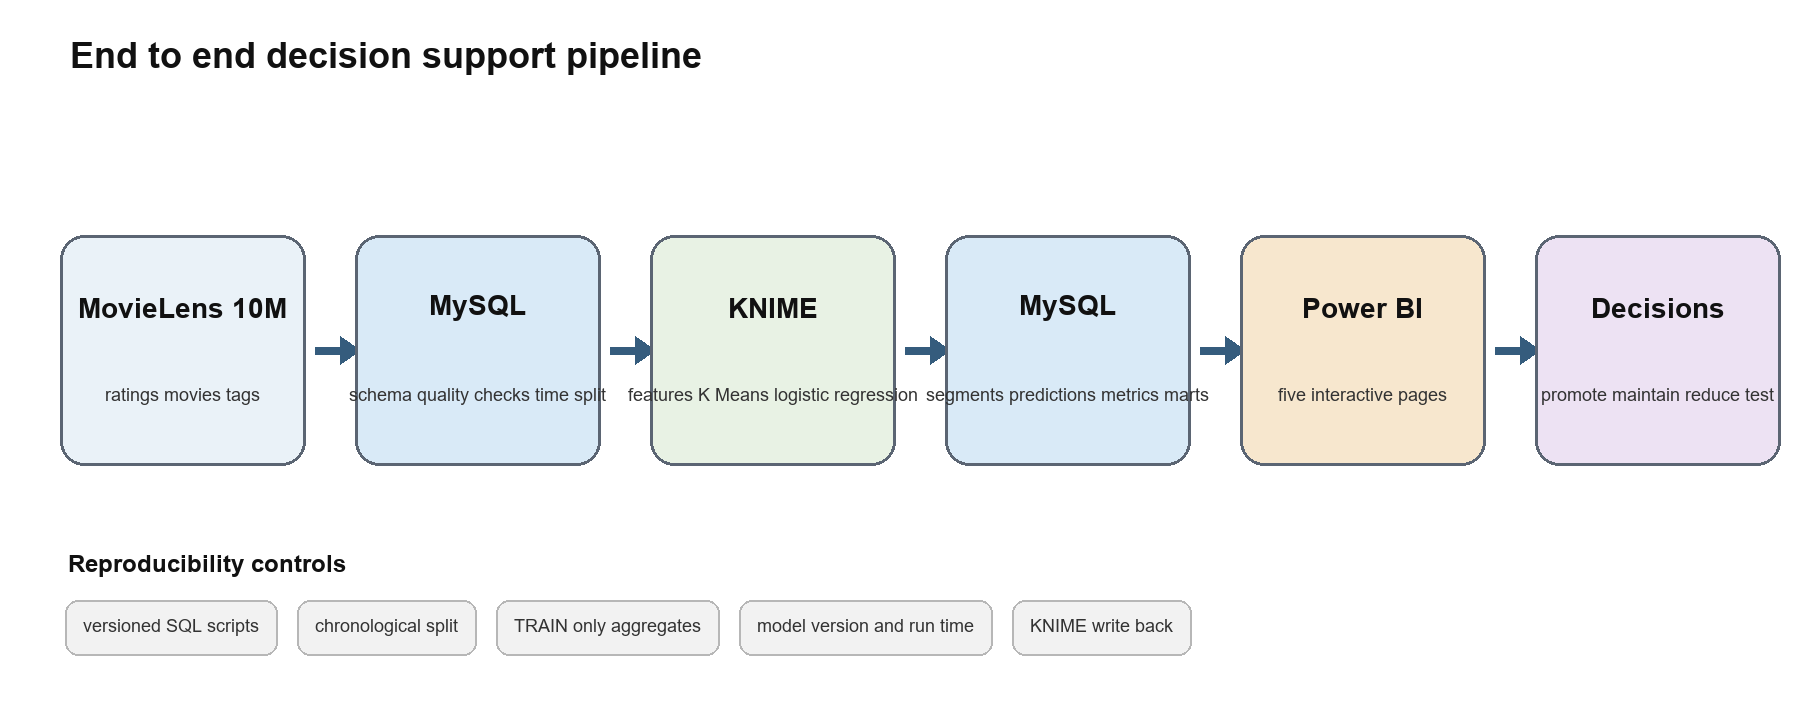
\includegraphics[width=0.92\textwidth]{architecture.png}
\caption{Implemented architecture from source files to decisions.}
\label{fig:arch}
\end{figure*}

\subsection{Data Quality Assessment}
Quality was checked in SQL and in the KNIME data-quality workflow for completeness, uniqueness, validity, consistency and plausible coverage. Table~\ref{tab:dq} reports the results. No rating row was invalid, duplicated or orphaned, so the interaction table was retained in full. The KNIME workflow standardises text attributes in separate tables without changing the source: titles are split into a clean title and release year, the \textit{(no genres listed)} label becomes a flag, tag text is trimmed and lower-cased, and whitespace-only tags are filtered out. Before and after values are written to a \texttt{dq\_summary} table.

\begin{table}[htbp]
\caption{Data quality before and after processing}
\label{tab:dq}
\centering
\begin{tabular}{@{}lrr@{}}
\toprule
Check & Before & After \\
\midrule
Rating rows & 10,000,054 & 10,000,054 \\
Orphan ratings or tags & 0 & 0 \\
Invalid ratings or timestamps & 0 & 0 \\
Duplicate user--movie pairs & 0 & 0 \\
Users below 20 ratings & 0 & 0 \\
Movies with at least one rating & 10,677 & 10,677 \\
\bottomrule
\end{tabular}
\end{table}

The remaining risks are conceptual rather than structural. Ratings are observed only when users choose to rate, the minimum of 20 ratings over-represents active users, the data end in 2009, and genre labels are broad and multi-valued.

\subsection{Chronological Split and Leakage Controls}
Ratings are ordered by timestamp and split 70/15/15 into TRAIN, VALID and TEST (Table~\ref{tab:split}). Four controls prevent leakage \cite{b10}. First, the split is chronological, so the model is always evaluated on a later period. Second, all user, movie and genre histories are computed from TRAIN only. Third, TRAIN rows use leave-one-out aggregates so that a rating is removed from its own predictors. Fourth, missing-value rules and z-score parameters are fitted on TRAIN and applied unchanged to VALID and TEST. User and movie identifiers are never used as numeric predictors.

\begin{table}[htbp]
\caption{Chronological split}
\label{tab:split}
\centering
\begin{tabular}{@{}lrl@{}}
\toprule
Split & Rows & Period \\
\midrule
TRAIN & 7,000,042 & 1995-01-09 to 2005-04-02 \\
VALID & 1,500,006 & 2005-04-02 to 2006-12-28 \\
TEST & 1,500,006 & 2006-12-28 to 2009-01-05 \\
\bottomrule
\end{tabular}
\end{table}

\subsection{K-Means Audience Segmentation}
Each user with TRAIN history is described by activity, length of rating history, average rating, rating dispersion, positive-rating rate and genre affinity. Affinity is the user's average rating for a genre minus the user's overall average, which separates a genuine genre preference from a generally generous rater. Features are standardised and K-Means \cite{b5} is run for $K=3,\dots,7$; the mean silhouette \cite{b6} guides the choice of $K$.

\subsection{Logistic Regression for Positive Engagement}
The target is $y=1$ when a rating is at least 4.0 and $y=0$ otherwise. The model estimates
\begin{equation}
P(y=1\mid \mathbf{x}) = \frac{1}{1+\exp\left(-\left(\beta_0+\boldsymbol{\beta}^{\top}\mathbf{x}\right)\right)},\label{eq:logit}
\end{equation}
where $\mathbf{x}$ contains the user's prior average rating, prior positive rate, activity, rating dispersion and active days; the movie's prior average rating, prior positive rate, popularity and dispersion; the user's segment; and 18 genre indicators. Activity, popularity and active days are log-transformed, and all numeric features are standardised on TRAIN. The model is trained in KNIME with the stochastic average gradient solver on a deterministic 20\% sample of TRAIN, checked on VALID, and evaluated once on TEST. A threshold of 0.5 converts \eqref{eq:logit} into a class. Final TEST metrics are recomputed in SQL from the stored predictions, so the dashboard and the paper use the same numbers.

Fig.~\ref{fig:knime} shows the KNIME workflow. Separate labelled sections handle TRAIN, VALID and TEST, the fitted missing-value and normaliser models are passed from the TRAIN branch to the other two, and a write-back section stores the TEST predictions and the coefficients in MySQL before an SQL node computes the metrics.

\begin{figure*}[!t]
\centering
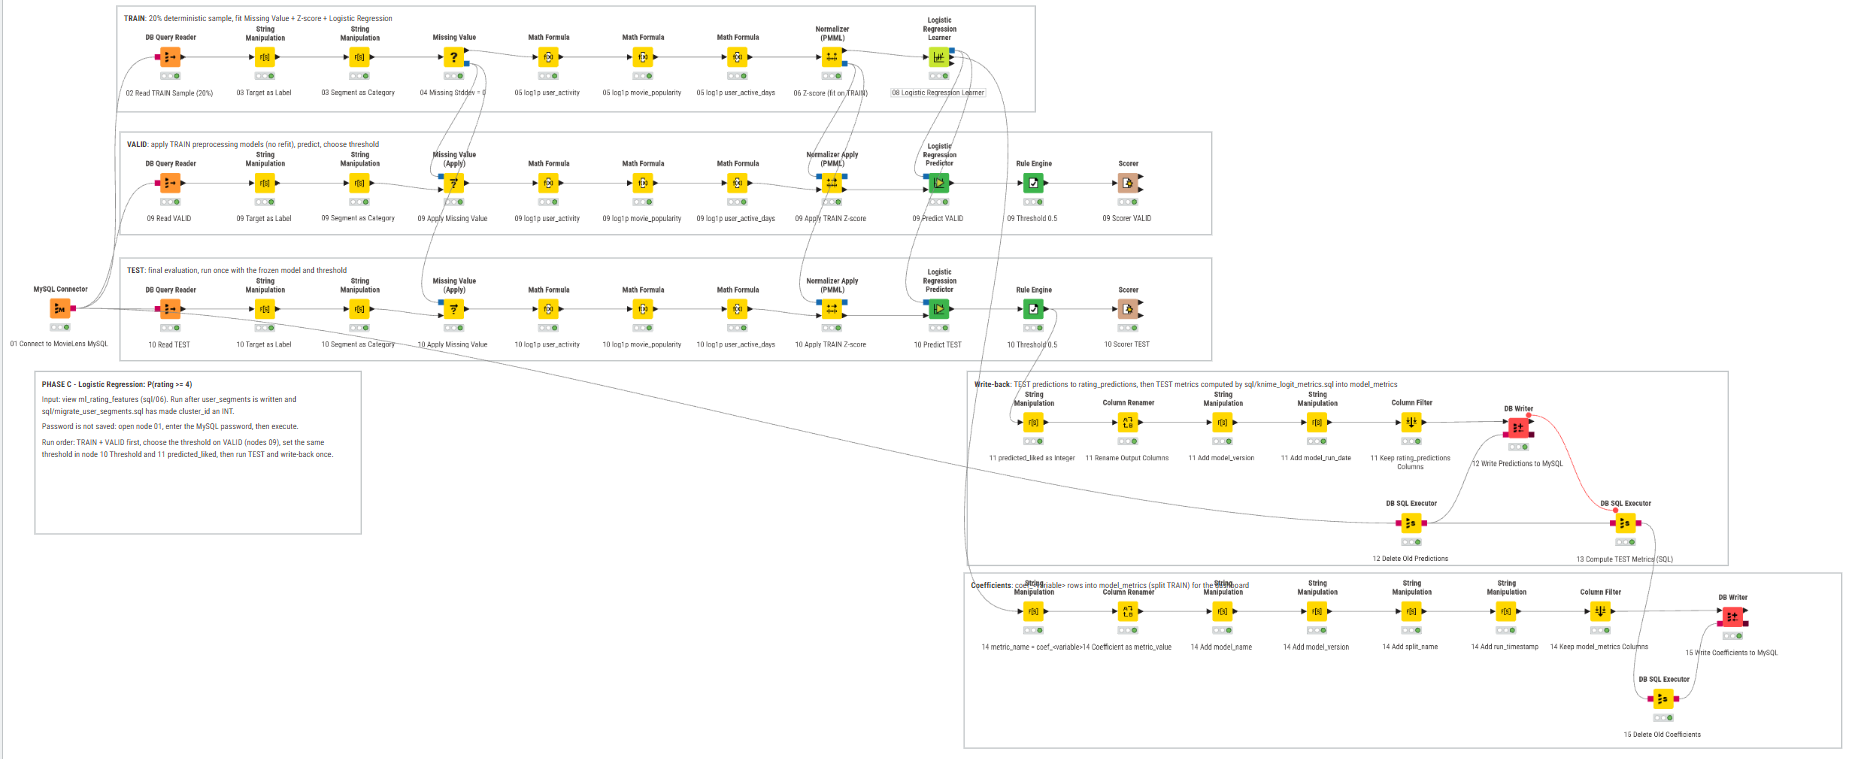
\includegraphics[width=0.95\textwidth]{knime_like_prediction.png}
\caption{KNIME Logistic Regression workflow: TRAIN, VALID and TEST branches with MySQL write-back of predictions, coefficients and metrics.}
\label{fig:knime}
\end{figure*}

A rating can be scored only if both the user and the movie have TRAIN history and the user has a segment. This warm-start rule protects the meaning of the features but limits coverage, which is therefore reported next to every metric.

\subsection{Reproducibility and Governance}
The repository contains the SQL and Python scripts, the three exported KNIME workflows, the Power BI file and a README. The pipeline is rebuilt in a fixed order: scripts 01 to 05 create the schema, load the data, run quality checks, build the split and compute TRAIN aggregates; the segmentation workflow writes \texttt{user\_segments}; script 06 builds the feature view; the Logistic Regression workflow writes predictions and metrics; and script 07 publishes the dashboard views before Power BI is refreshed. Credentials are kept in an ignored environment file or in KNIME credential settings, so no password is stored in the repository. Every result row carries a model version and run time, and the dashboard filters on a single version, which prevents rows from different runs from being combined.

\section{Experiments and Results}

\subsection{Exploratory Analysis}
Rating 4.0 is the most frequent value with 2,875,850 occurrences (Fig.~\ref{fig:dist}). Drama has the largest volume, 4,344,198 ratings, with a 56.52\% positive rate, whereas Film-Noir reaches 71.95\% on far fewer ratings. A high positive rate on its own is therefore not a sufficient promotion rule; support must be considered.

\begin{figure}[htbp]
\centering
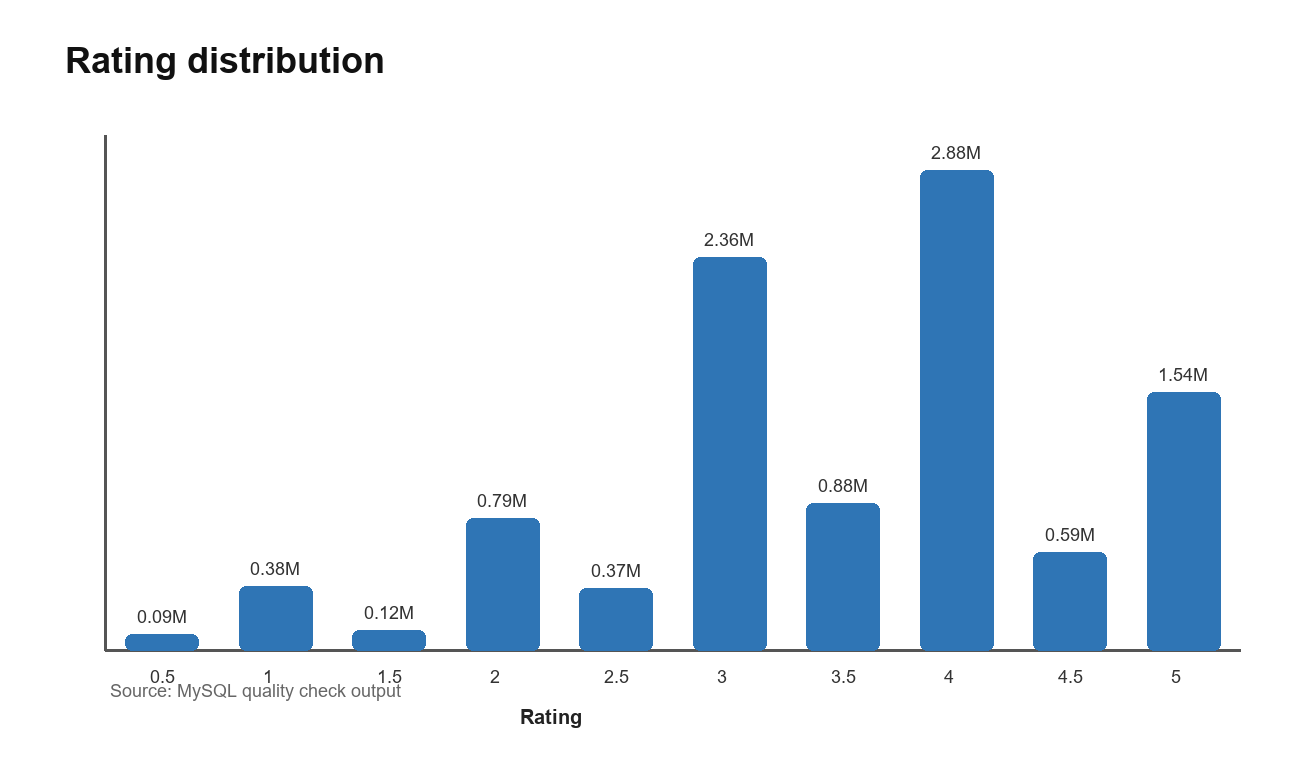
\includegraphics[width=\columnwidth]{rating_distribution.png}
\caption{Distribution of all 10,000,054 ratings.}
\label{fig:dist}
\end{figure}

\subsection{Audience Segments}
Table~\ref{tab:sil} lists the silhouette scores. $K=5$ is only 0.00055 above $K=4$, so $K=4$ was kept because it gives one fewer profile to explain with almost identical separation. The absolute scores are low, which means the segments overlap and should be read as behavioural lenses rather than natural groups.

\begin{table}[htbp]
\caption{Mean silhouette by number of clusters}
\label{tab:sil}
\centering
\begin{tabular}{@{}ccccc@{}}
\toprule
$K=3$ & $K=4$ & $K=5$ & $K=6$ & $K=7$ \\
\midrule
0.0602 & \textbf{0.0686} & 0.0692 & 0.0646 & 0.0651 \\
\bottomrule
\end{tabular}
\end{table}

The four segments cover 54,873 of the 69,878 rating users (Fig.~\ref{fig:clusters}). Genre Specialists are the largest group, 17,346 users, with the highest positive-rating rate of 71.43\%. Mainstream Enthusiasts, 14,457 users, show relative family and animation affinity and the lowest positive rate, 42.06\%. Diverse Explorers, 12,182 users, show relative thriller, action and mystery affinity with a 51.38\% positive rate. Selective Critics, 10,888 users, average 385.3 TRAIN ratings per user, compared with roughly 61 to 67 in the other segments, and have a 50.88\% positive rate.

\begin{figure}[htbp]
\centering
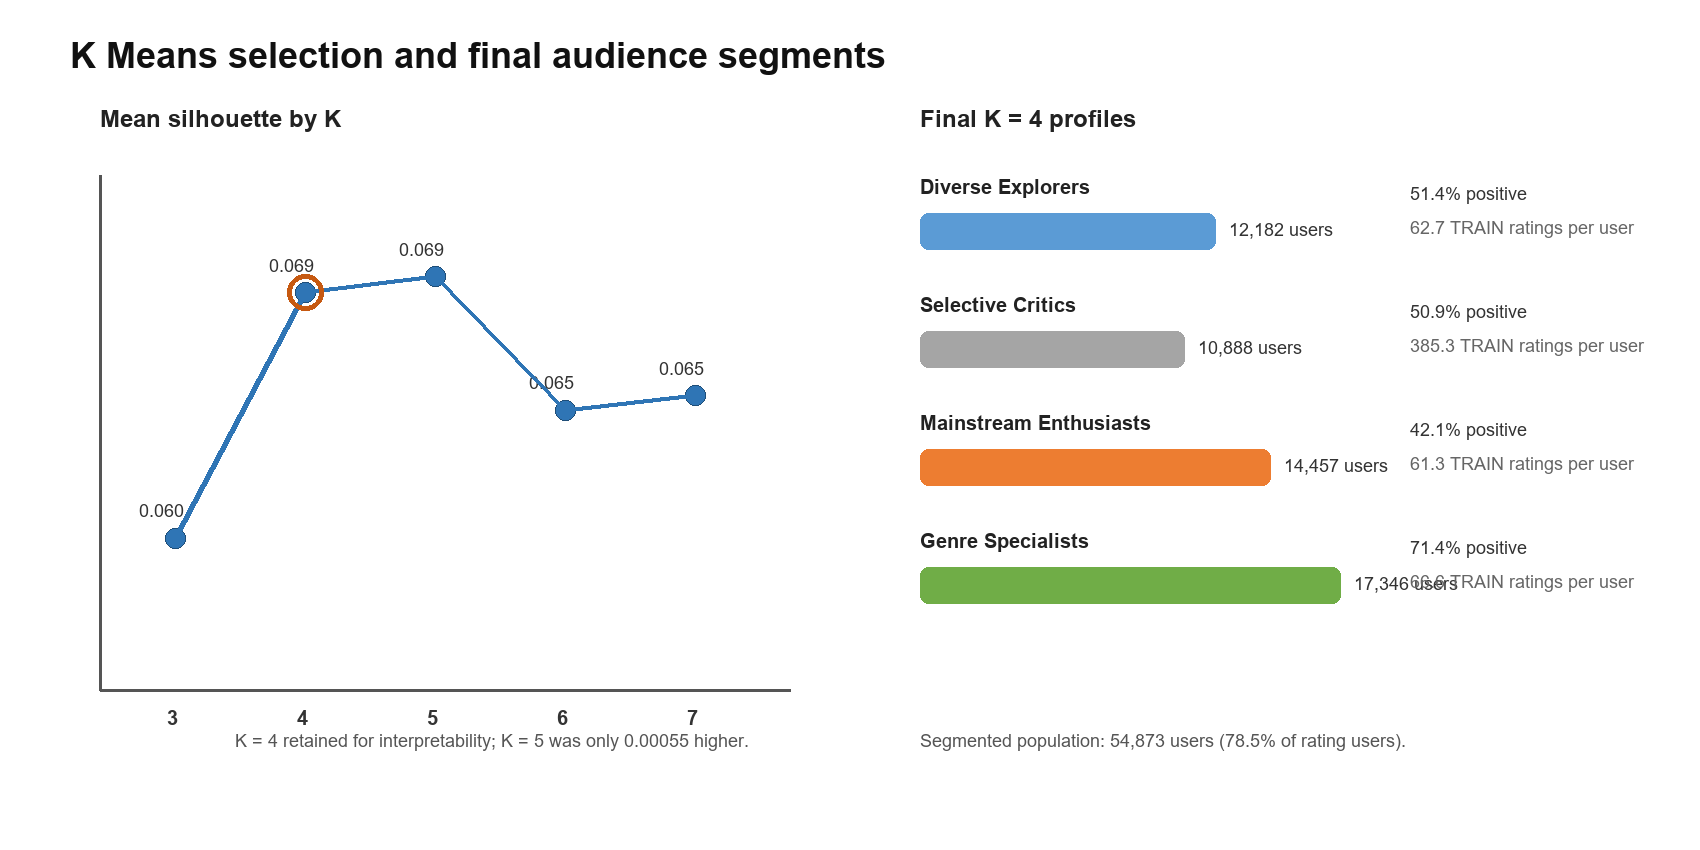
\includegraphics[width=\columnwidth]{clustering_summary.png}
\caption{Silhouette by $K$ and size of the four final segments.}
\label{fig:clusters}
\end{figure}

\subsection{Positive-Engagement Model}
Table~\ref{tab:metrics} reports the TEST results. Accuracy is 9.93 percentage points above the majority baseline, and the ROC-AUC of 0.758 shows useful ranking ability \cite{b8}. The confusion matrix contains 31,273 true negatives, 14,189 false positives, 9,369 false negatives and 21,802 true positives (Fig.~\ref{fig:model}). In a promotion setting a false positive wastes a display slot and a false negative is a missed discovery, so recall of 69.94\% with precision of 60.58\% suits a candidate-generation role that is followed by testing. The largest standardised coefficients belong to the user's prior positive rate, the movie's prior average rating and the movie's prior positive rate, so prior behaviour drives predictions more than genre or segment membership.

\begin{table}[htbp]
\caption{Logistic Regression results on TEST}
\label{tab:metrics}
\centering
\begin{tabular}{@{}lr@{}}
\toprule
Metric & Value \\
\midrule
Accuracy & 69.26\% \\
Majority baseline & 59.32\% \\
Precision & 60.58\% \\
Recall & 69.94\% \\
F1 & 64.92\% \\
ROC-AUC & 0.758 \\
Scored TEST rows & 76,633 of 1,500,006 (5.11\%) \\
\bottomrule
\end{tabular}
\end{table}

\begin{figure}[htbp]
\centering
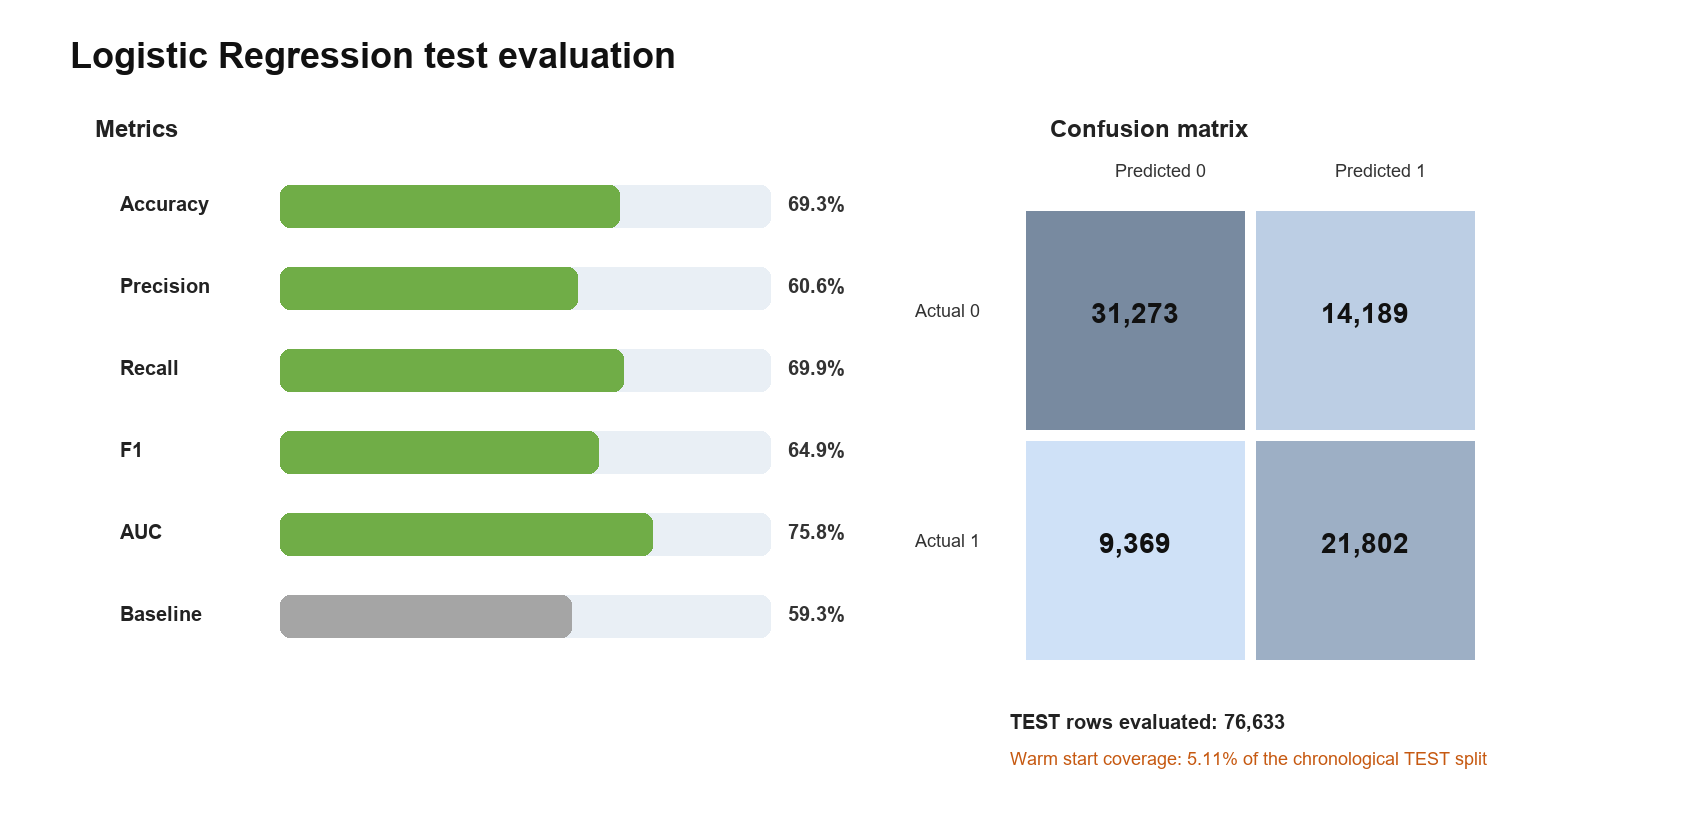
\includegraphics[width=\columnwidth]{model_evaluation.png}
\caption{TEST metrics and confusion matrix of the Logistic Regression model.}
\label{fig:model}
\end{figure}

Coverage is the main limitation. Because TEST runs from late 2006 to 2009 and TRAIN ends in April 2005, most TEST ratings come from users or movies without TRAIN history, and 94.89\% of TEST rows are excluded by the warm-start rule. This is the cold-start problem described by Schein et al. \cite{b4}. The metrics therefore describe the eligible subset only.

\subsection{Interactive Dashboard}
The Power BI report has five pages, each answering one question: Executive Overview (is the evidence base usable), Audience Segments (who are the segments), Positive Engagement Model (how good is the model and where), Content Opportunity Matrix (which titles to promote or test) and Model Governance (when results are safe to use). Global slicers for model version, segment, genre and minimum TEST support prevent mixing model runs or reading weak cells. Fig.~\ref{fig:dash} shows two pages.

\begin{figure}[H]
\centering
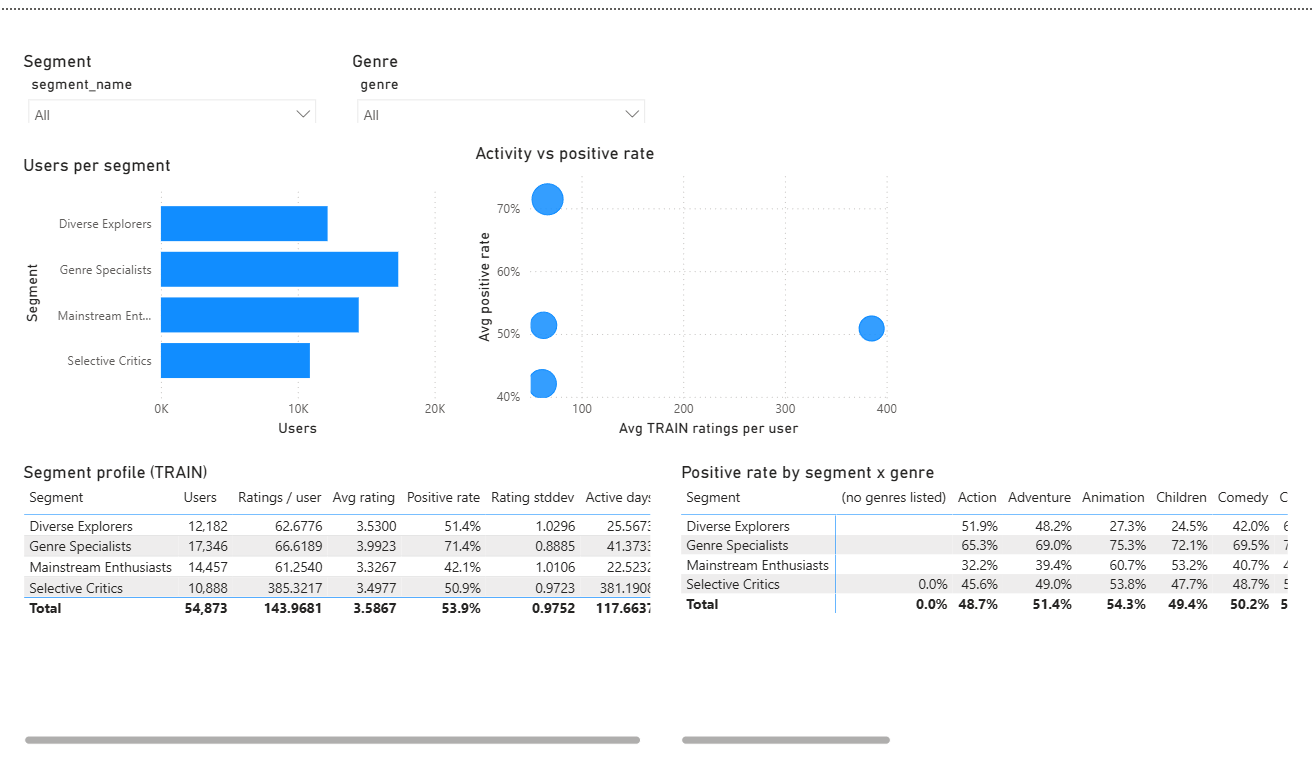
\includegraphics[width=\columnwidth]{dashboard_segments.png}
\vspace{1mm}
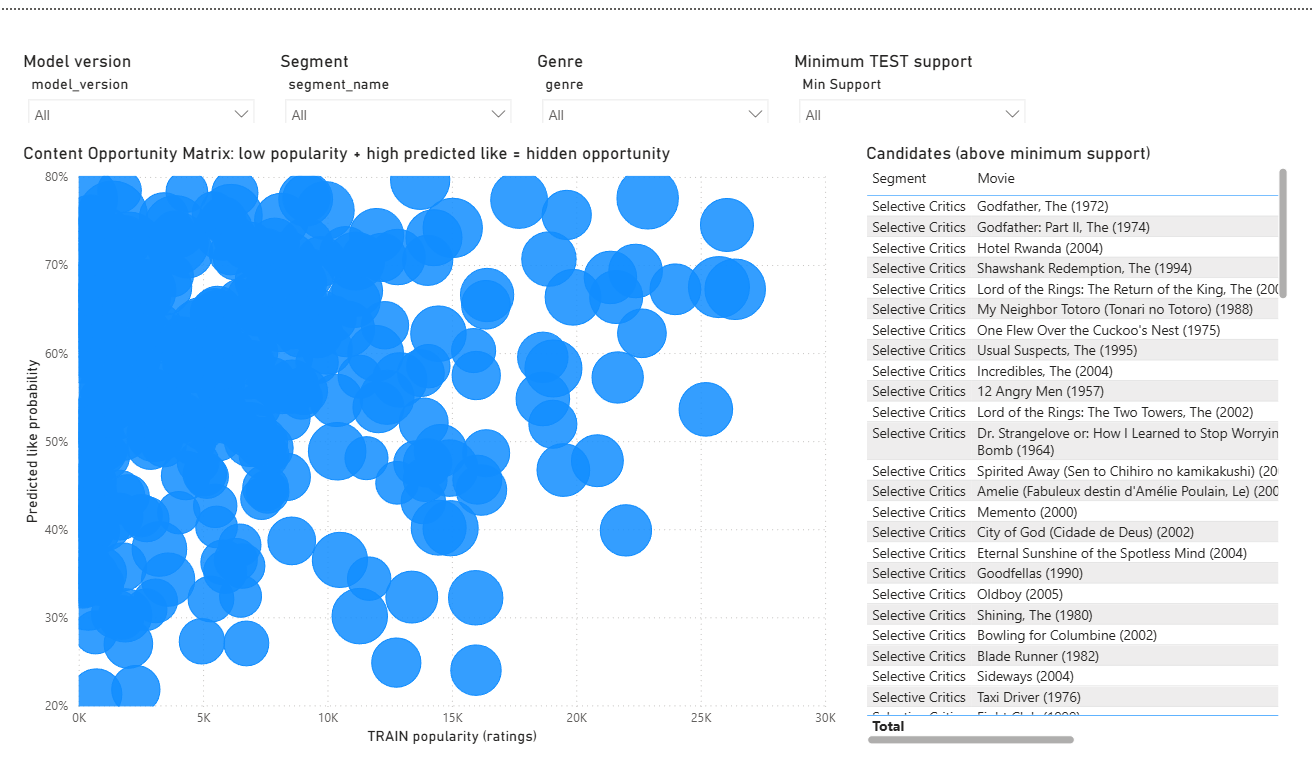
\includegraphics[width=\columnwidth]{dashboard_opportunity.png}
\caption{Power BI pages for Audience Segments (top) and the Content Opportunity Matrix (bottom).}
\label{fig:dash}
\end{figure}

\subsection{Content Opportunities}
The opportunity matrix compares predicted appeal with TRAIN popularity, with TEST support as bubble size (Fig.~\ref{fig:opp}). Only Selective Critics produced title--segment pairs with TEST support of at least 50, 107 pairs in total; the other segments peaked between 18 and 30 ratings per title and are treated as exploratory. Table~\ref{tab:opp} lists the strongest low-popularity candidates, whose predicted and observed positive rates agree closely. In contrast, Home Alone, Star Wars Episode I, Twister and The Mask have support above 50 but observed positive rates of only 17.65\%, 19.61\%, 10.17\% and 5.66\% in this segment. The Incredibles is a calibration warning: predicted 74.45\% against an observed 60.75\% over 107 ratings.

\begin{table}[htbp]
\caption{Hidden opportunities for Selective Critics}
\label{tab:opp}
\centering
\begin{tabular}{@{}lrrrr@{}}
\toprule
Title & Supp. & Pred. & Actual & Pop. \\
\midrule
Hotel Rwanda & 108 & 76.72\% & 77.78\% & 215 \\
My Neighbor Totoro & 58 & 74.87\% & 74.14\% & 487 \\
City of God & 60 & 71.66\% & 70.00\% & 968 \\
Oldboy & 52 & 69.94\% & 67.31\% & 72 \\
\bottomrule
\end{tabular}
\end{table}

\begin{figure}[H]
\centering
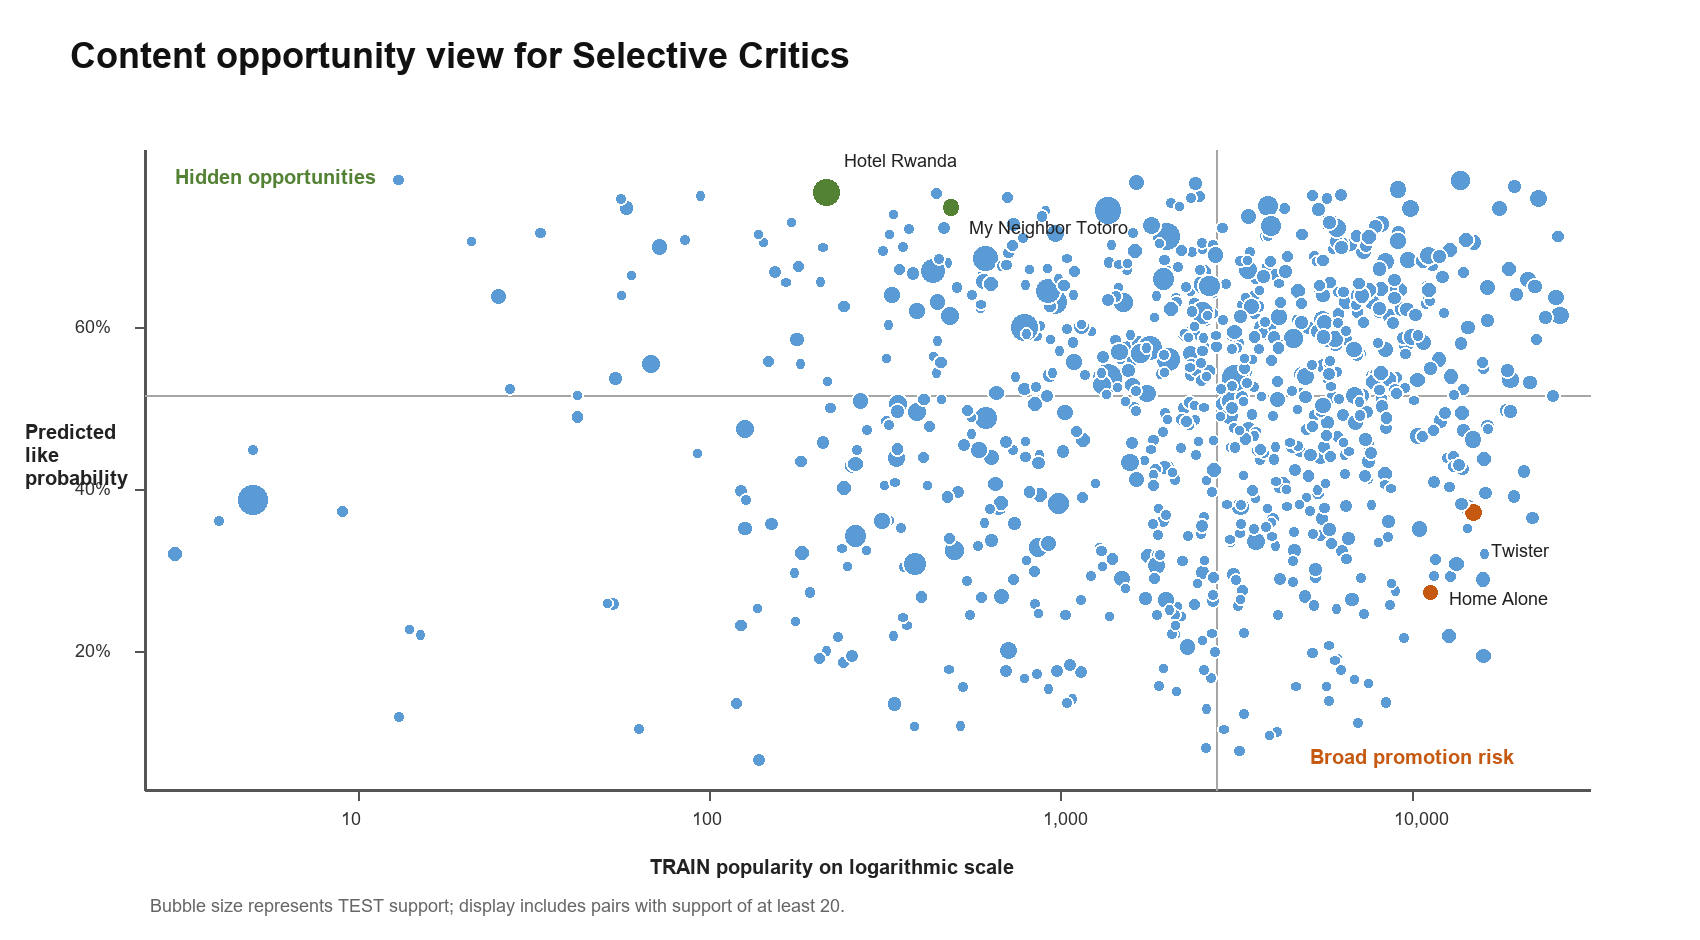
\includegraphics[width=\columnwidth]{content_opportunity.png}
\caption{Content opportunity matrix for Selective Critics.}
\label{fig:opp}
\end{figure}

\section{Discussion and Decision Recommendations}
\subsection{Answers to the Decision Questions}
\textit{Question 1.} Rating behaviour differs mainly in activity and generosity: one segment rates about six times more than the others, and positive-rating rates range from 42.06\% to 71.43\% across segments, with distinct relative genre preferences.

\textit{Question 2.} Four segments are interpretable and each contains more than 10,000 users, but the low silhouette means they should guide curation hypotheses rather than fixed targeting rules.

\textit{Question 3.} Prior user and movie behaviour identify positive ratings with 69.26\% accuracy and 0.758 ROC-AUC, a clear gain over the baseline, but only for the 5.11\% of test ratings with warm-start history.

\textit{Question 4.} Hotel Rwanda, My Neighbor Totoro, City of God and Oldboy combine low TRAIN popularity with high and well-calibrated predicted appeal for Selective Critics, which makes them the first candidates for a controlled test.

\subsection{Recommendations}
The evidence supports bounded actions rather than automated promotion. Table~\ref{tab:rec} lists four recommendations with their evidence, expected benefit and main risk.

\begin{table*}[!t]
\caption{Evidence-based recommendations}
\label{tab:rec}
\centering
\begin{tabular}{@{}p{0.22\textwidth}p{0.30\textwidth}p{0.20\textwidth}p{0.20\textwidth}@{}}
\toprule
Action & Evidence & Expected benefit & Assumptions and risks \\
\midrule
1. Test Hotel Rwanda and My Neighbor Totoro in a discovery row for Selective Critics & Support 108 and 58; predicted 76.72\% and 74.87\% against observed 77.78\% and 74.14\%; TRAIN popularity 215 and 487 & More discovery of under-exposed titles with aligned predicted and observed appeal & Rating is a proxy for satisfaction; warm-start users only; requires an A/B test \\
\addlinespace
2. Add City of God and Oldboy to the same candidate pool & Support 60 and 52; predicted 71.66\% and 69.94\% against observed 70.00\% and 67.31\%; popularity 968 and 72 & Broader slate beyond blockbusters for the most active segment & Small support gives wide intervals; monitor each title \\
\addlinespace
3. Reduce default placement of Home Alone, Star Wars Episode I, Twister and The Mask for this segment & Support above 50 with observed positive rates of 17.65\% to 5.66\% despite high popularity & Less segment-specific mismatch; slots reallocated to better-fitting titles & Titles stay in the catalogue; watch diversity and engagement loss \\
\addlinespace
4. Use segment-aware ranking only where warm-start evidence exists, with a popularity or editorial fallback & Classifier TEST coverage 5.11\%; segments cover 54,873 of 69,878 users (78.5\%) & Avoids unsupported predictions; coverage tracked as a deployment KPI & Fallback quality is not measured by this model \\
\bottomrule
\end{tabular}
\end{table*}

Model scores do not establish that a campaign will change behaviour. Following Kohavi et al. \cite{b11}, eligible users should be randomly assigned to the current experience or to the segment-specific slate, with the same placement, time window and exposure. Positive-rating rate is the primary measure available here; click-through, play start, completion and revenue should replace it when such data exist. Confidence intervals and a minimum sample size should be fixed before the test.

The main threats to validity are temporal drift between 2005 and 2009, selection bias towards active raters, unobserved exposure, overlapping clusters with low silhouette, untested probability calibration and the narrow warm-start coverage. Promising improvements are cold-start features from genres and tags, probability calibration, ranking metrics such as precision at $k$ \cite{b9}, rolling temporal validation and comparison with a latent factor model \cite{b3}.

\section{Conclusion}
This work delivers a complete decision-support chain for segment-based movie promotion. MovieLens 10M is stored and validated in MySQL, processed and modelled in KNIME with results written back to MySQL, and presented in an interactive Power BI dashboard. K-Means provides four interpretable but overlapping audience lenses, and Logistic Regression improves accuracy by 9.93 percentage points over the majority baseline with a ROC-AUC of 0.758 on eligible test ratings. Because only 5.11\% of the test period is covered, the system is best used to prioritise transparent, measurable experiments for warm-start users, starting with Selective Critics, while popularity or editorial rules serve everyone else.

\begin{thebibliography}{00}
\bibitem{b1} GroupLens Research, ``MovieLens 10M dataset and README,'' 2009. [Online]. Available: \url{https://grouplens.org/datasets/movielens/10m/}
\bibitem{b2} F. M. Harper and J. A. Konstan, ``The MovieLens datasets: History and context,'' \textit{ACM Trans. Interact. Intell. Syst.}, vol. 5, no. 4, pp. 19:1--19:19, 2015.
\bibitem{b3} Y. Koren, R. Bell, and C. Volinsky, ``Matrix factorization techniques for recommender systems,'' \textit{Computer}, vol. 42, no. 8, pp. 30--37, 2009.
\bibitem{b4} A. I. Schein, A. Popescul, L. H. Ungar, and D. M. Pennock, ``Methods and metrics for cold-start recommendations,'' in \textit{Proc. 25th Annu. Int. ACM SIGIR Conf. Research and Development in Information Retrieval}, 2002, pp. 253--260.
\bibitem{b5} S. P. Lloyd, ``Least squares quantization in PCM,'' \textit{IEEE Trans. Inf. Theory}, vol. 28, no. 2, pp. 129--137, 1982.
\bibitem{b6} P. J. Rousseeuw, ``Silhouettes: A graphical aid to the interpretation and validation of cluster analysis,'' \textit{J. Comput. Appl. Math.}, vol. 20, pp. 53--65, 1987.
\bibitem{b7} D. W. Hosmer, S. Lemeshow, and R. X. Sturdivant, \textit{Applied Logistic Regression}, 3rd ed. Hoboken, NJ, USA: Wiley, 2013.
\bibitem{b8} T. Fawcett, ``An introduction to ROC analysis,'' \textit{Pattern Recognit. Lett.}, vol. 27, no. 8, pp. 861--874, 2006.
\bibitem{b9} A. Gunawardana and G. Shani, ``A survey of accuracy evaluation metrics of recommendation tasks,'' \textit{J. Mach. Learn. Res.}, vol. 10, pp. 2935--2962, 2009.
\bibitem{b10} S. Kaufman, S. Rosset, C. Perlich, and O. Stitelman, ``Leakage in data mining: Formulation, detection, and avoidance,'' \textit{ACM Trans. Knowl. Discov. Data}, vol. 6, no. 4, pp. 15:1--15:21, 2012.
\bibitem{b11} R. Kohavi, R. Longbotham, D. Sommerfield, and R. M. Henne, ``Controlled experiments on the web: Survey and practical guide,'' \textit{Data Min. Knowl. Discov.}, vol. 18, no. 1, pp. 140--181, 2009.
\bibitem{b12} M. R. Berthold \textit{et al.}, ``KNIME -- the Konstanz Information Miner: Version 2.0 and beyond,'' \textit{ACM SIGKDD Explor. Newsl.}, vol. 11, no. 1, pp. 26--31, 2009.
\end{thebibliography}

\end{document}
